
    \documentclass{standalone}
\usepackage{tkz-fct}
\usepackage{tkz-euclide}
\usepackage{color}
\renewcommand*\familydefault{\sfdefault}
\usepackage{sansmath}
\sansmath
\definecolor{gray75}{gray}{0.75}
\begin{document}
 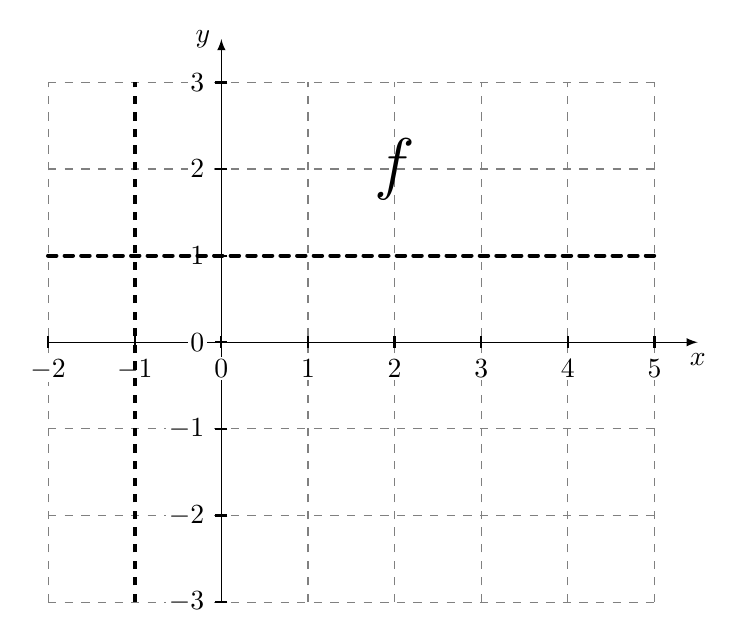
\begin{tikzpicture}[scale=1.1]
   \tkzInit[xmax=5.0,ymax=3.0,xmin=-2.0 ,ymin=-3.0]
   \begin{scope}[dashed]
     \tkzGrid
   \end{scope}
   \tkzDrawX[label={$x$}]
   \tkzDrawY[label={$y$}]
   \tkzLabelX
   \tkzLabelY
   \tkzFctPar[line width=2pt,samples=400,domain=0:1]{((21491177421812014*t**3 + 32166869290015563*t**2 + 69896842702440*t - 8691947280825057)/9007199254740992)}{(3*(2389910202257943*t**3 - 10394503237101085*t**2 + 13979368540488000*t - 4503599627370496)/4503599627370496)}

   
                \tkzDefPoint(-2.0,1.0){A}

                \tkzDefPoint(5.0,1.0){B}

                \tkzDrawSegment[style=dashed,line width = 1.5pt](A,B)

                \tkzVLine[style=dashed,line width = 1.5pt]{-1.0}

   

   \tkzText(2,2){\Huge$f$}

\end{tikzpicture}
\end{document}

    